In this chapter, we will test the running time of traditional QR Algorithm and Aggressive Early Defaltion, and the numerical stability. The test source code see \textbf{The Appendix B} and all matrices are initially generated by the build-in \(rand\) and each element is between-1 and 1
First, we test the performance of The Double-Shift-QR-Algorithm and Sextuple-Shift-QR-Algorithm, select a matrix from 110 to 1000 and select one every 10.
\begin{figure}[H]
\centering
\includegraphics{The running time of traditional QR Algorithm.eps}
\caption{The running time of traditional QR Algorithm}
\label{1}
\end{figure}

This test can shows us that selecting more shifts every time can improve efficiency, so we propose multishift QR Algorithm, and choose small-bugle, which introduced two shifts each time. Then, add Aggressive Early Defaltion in and test again. This time it ranges from 620 to 1200 (since AED does not improve performance significantly in small matrices).
\begin{figure}[H]
\centering
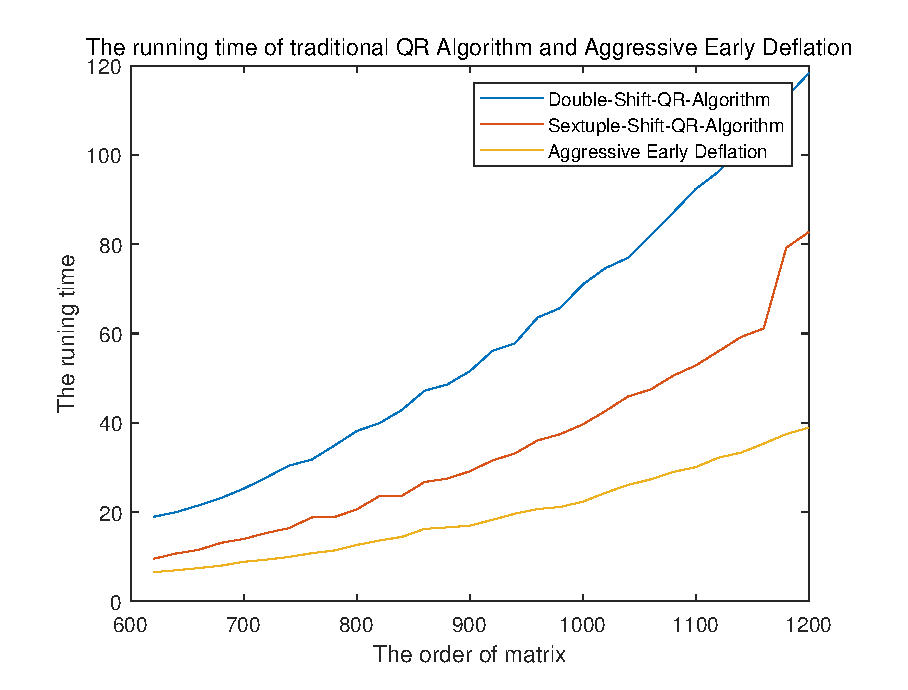
\includegraphics[height=10cm,width=15cm]{The running time of traditional QR Algorithm and Aggressive Early Deflation.eps}
\caption{The running time of traditional QR Algorithm and Aggressive Early Deflation}
\label{2}
\end{figure}

In the exploration function of Matlab, we can see that when the matrix order reaches 1000, the time required for hessenberg is close to that for AED processing. Now, we do a numerical experiment to prove it.
\begin{figure}[H]
\centering
\includegraphics[height=10cm,width=15cm]{Hessenberg.eps}
\caption{The running time of Hessenberg and Matlab function}
\label{3}
\end{figure}

This can prove that the hessenberg program written by myself does not use BLAS-3 performance when dealing with thousands of matrices, so the performance will be much worse. Then, I use the built-in function \(hess\) to do following test.

Then we test Aggressive Early Defaltion with \(hess\) and the built-in function \(schur\), select a matrix from 1000 to 5350 and select one every 150.
\begin{figure}[H]
\centering
\includegraphics[height=10cm]{The running time of the Aggressive Early Deflation.eps}
\caption{The running time of the Aggressive Early Deflation}
\label{4}
\end{figure}

This test can shows us we can do a real-schur decomposition for a 5000*5000 matrix in about 6 minutes, then let us see the numerical stability.

We choose 23 matrices of order 500, change their condition number from \(10^3\) to \(10^14\) by singular value decomposition, then compute \(\frac{{{{\left\| {AQ - QH} \right\|}_F}}}{{{{\left\| A \right\|}_F}}}\) and \(\frac{{{{\left\| {{Q^T}Q - I} \right\|}_F}}}{{\sqrt n }}\) Then we can get:
\begin{figure}[H]
  \centering
  \subfigure[The numerical stability for schur decomposition]{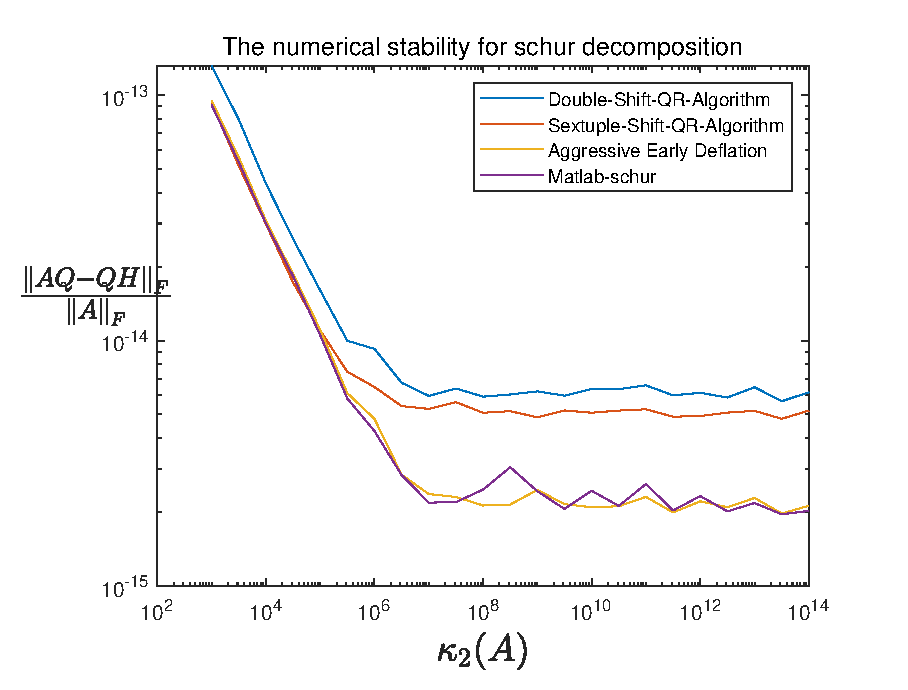
\includegraphics[width=3in]{The numerical stability for schur decomposition.eps}}
  \subfigure[The numerical stability for orthogonal matrix]{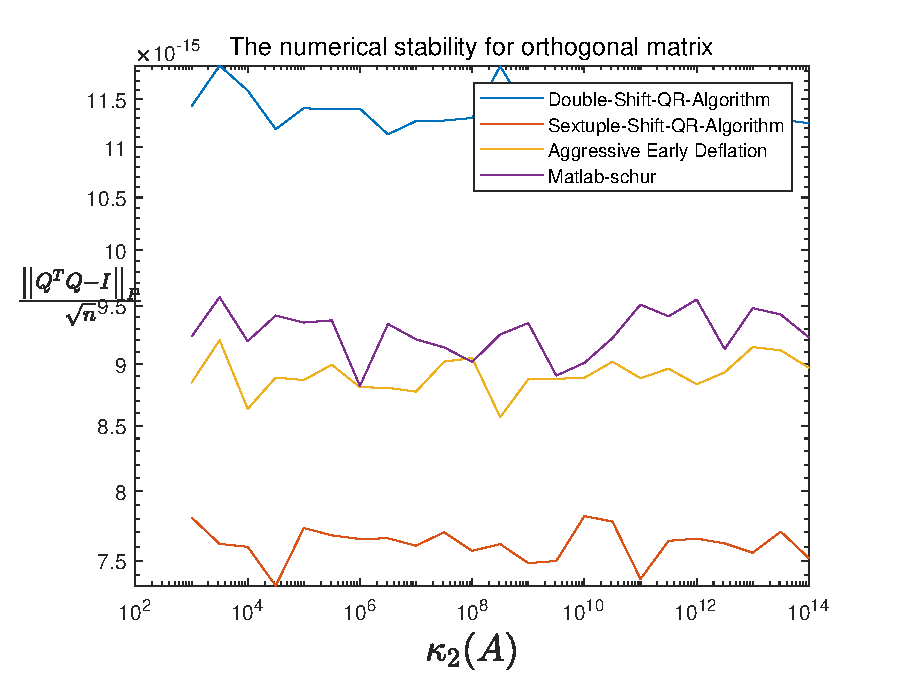
\includegraphics[width=3in]{The numerical stability for orthogonal matrix.eps}}
  \caption{The numerical stability}
\end{figure}

This can show us that the numerical stability is enough. I think maybe because of every orthogonal transformation is made with a home transformation.

As a reference standard, the information about the computer and the time to run the schur decomposition of the built-in matlab function will be given in the \textbf{The Appendix A} and all the matlab source code will be given in the \textbf{The Appendix B}.